\begin{frame}
    \frametitle{\problemtitle}
    \begin{block}{Problem}
      Given are $5$ locations in a city grid with square blocks.
      Refurbish a set of streets in the grid such that
      \begin{itemize}
        \item for any two locations there exists a shortest path between them that only uses refurbished streets;
        \item the total length of the refurbished streets is minimized.
      \end{itemize}
      Output the minimal total length.
    \end{block}
    \centering
    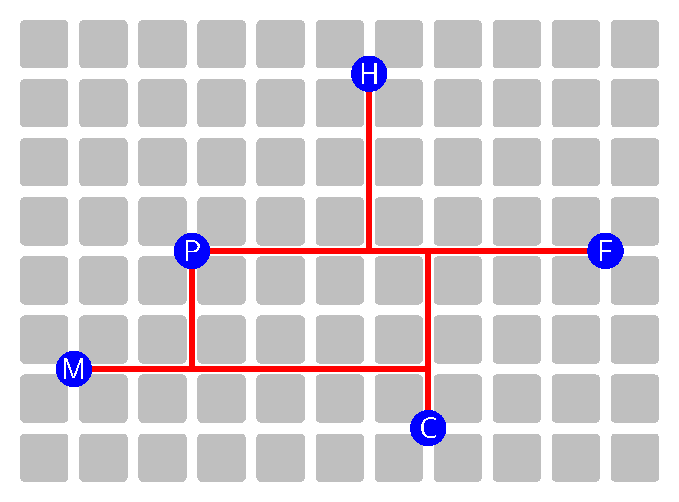
\includegraphics[width=0.4\textwidth]{sol1.pdf}
\end{frame}
\begin{frame}
    \frametitle{\problemtitle}
    \begin{block}{Insight}
      If there is a unique leftmost point, we may refurbish a street towards
      the right, then relocate that point along that street.
      The same reasoning applies on the right, top or bottom.
    \end{block}
    \centering
    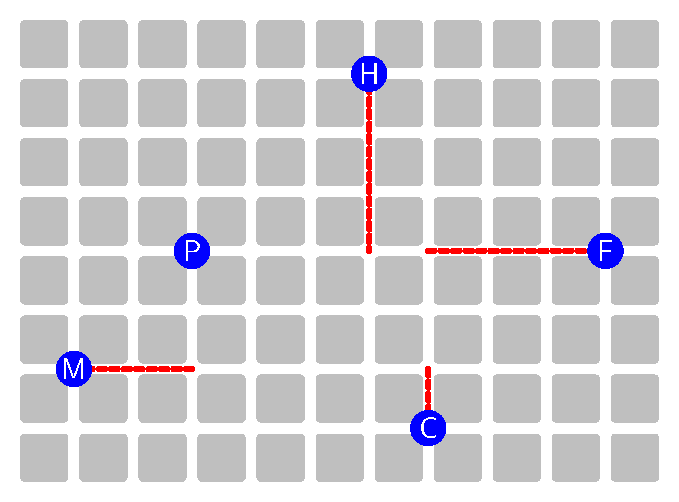
\includegraphics[width=0.4\textwidth]{sol2.pdf}%
    \hspace{1cm}%
    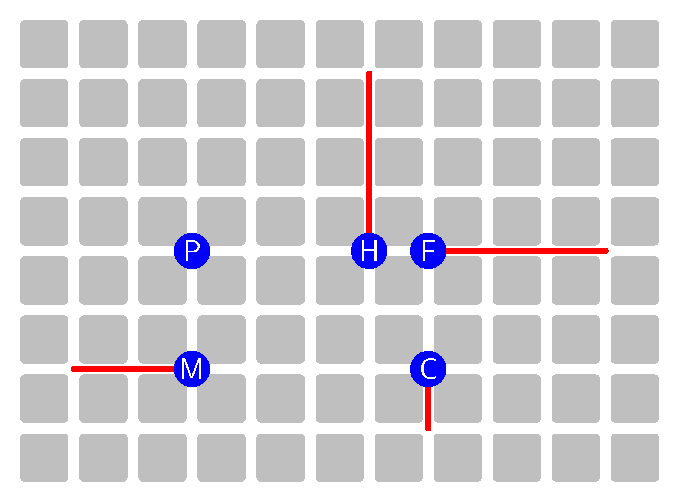
\includegraphics[width=0.4\textwidth]{sol3.pdf}
\end{frame}
\begin{frame}
    \frametitle{\problemtitle}
    \begin{block}{Solution}
      \begin{itemize}
        \item Repeat this action until this is no longer possible. Remove duplicates after each step.
        \item This leaves either a single point or one of the scenarios below (up to symmetry).
        \item The remaining solution is now a rectangle, maybe with an extra chord.
      \end{itemize}
    \end{block}
    \begin{center}
      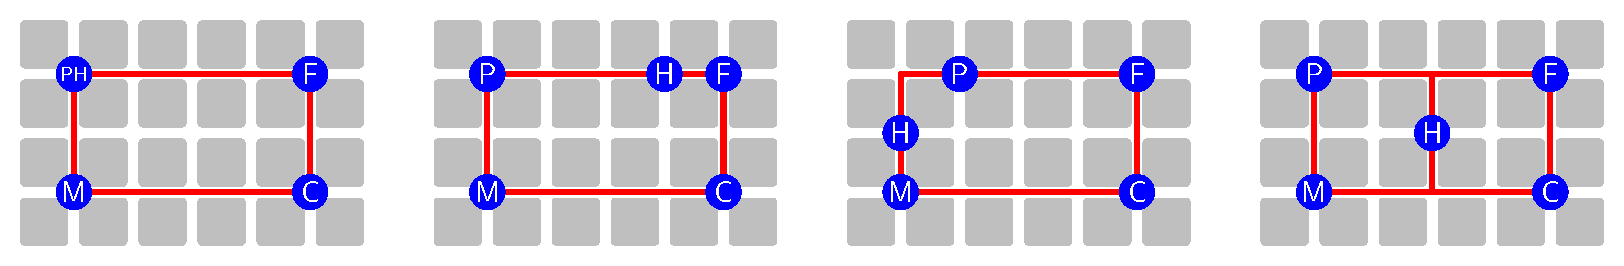
\includegraphics[width=0.96\textwidth]{sol4.pdf}
    \end{center}
    \pause
    \solvestats
\end{frame}
